\documentclass[xetex, aspectratio=169, russian]{beamer}
\beamertemplatenavigationsymbolsempty
\setbeamertemplate{footline}[frame number]

\usepackage{fontspec}
\usepackage{polyglossia}
\usepackage[autostyle]{csquotes}
\setmainlanguage[babelshorthands]{russian}
\setotherlanguage{english}

\setmainfont{CMU Serif}
\setsansfont{CMU Sans Serif}
\setmonofont{CMU Typewriter Text}

\usepackage{booktabs}
\usepackage{multirow}
\usepackage{makecell}
\usepackage{ltablex}
\usepackage{paralist}
\keepXColumns
\renewcommand\theadfont{\normalsize}

\usepackage{fvextra}
\usepackage{xcolor}
\usepackage{textcomp}
\usepackage{graphicx}
\usepackage[edges]{forest}
\graphicspath{{../img/}}

\usepackage{mathtools}
\usepackage{amssymb}

\usepackage{covington}
\renewcommand*\glosslinetrans[1]{`#1'}

% Библиография
\usepackage[
    backend=biber,
    bibencoding=utf8,
    style=gost-authoryear,
    language=auto,
    autolang=other,
    clearlang=true,
    sortcites=true,
    movenames=false,
    minbibnames=3,
    maxbibnames=5
]{biblatex}

% Сортировка библиографии
\DeclareSourcemap{
    \maps[datatype=bibtex]{
        \map{
            \step[fieldsource=langid, match=russian, final]
            \step[fieldset=presort, fieldvalue={a}]
        }
        \map{
            \step[fieldsource=langid, notmatch=russian, final]
            \step[fieldset=presort, fieldvalue={z}]
        }
    }
}

% Убираем неразрывные пробелы перед двоеточием и точкой с запятой
\makeatletter

\renewcommand*{\addcolondelim}{%
    \begingroup%
    \def\abx@colon{%
        \ifdim\lastkern>\z@\unkern\fi%
        \abx@puncthook{:}\space}%
    \addcolon%
    \endgroup%
}

\renewcommand*{\addsemicolondelim}{%
    \begingroup%
    \def\abx@semicolon{%
        \ifdim\lastkern>\z@\unkern\fi%
        \abx@puncthook{;}\space}%
    \addsemicolon%
    \endgroup%
}

\makeatother

% Правка записей типа thesis, чтобы дважды не писался автор
\DeclareBibliographyDriver{thesis}{%
    \usebibmacro{bibindex}%
    \usebibmacro{begentry}%
    \usebibmacro{heading}%
    \newunit
    \usebibmacro{author}%
    \setunit*{\labelnamepunct}%
    \usebibmacro{thesistitle}%
    \setunit{\respdelim}%
    \newunit\newblock
    \printlist[semicolondelim]{specdata}%
    \newunit
    \usebibmacro{institution+location+date}%
    \newunit\newblock
    \usebibmacro{chapter+pages}%
    \newunit
    \printfield{pagetotal}%
    \newunit\newblock
    \usebibmacro{doi+eprint+url+note}%
    \newunit\newblock
    \usebibmacro{addendum+pubstate}%
    \setunit{\bibpagerefpunct}\newblock
    \usebibmacro{pageref}%
    \newunit\newblock
    \usebibmacro{related:init}%
    \usebibmacro{related}%
    \usebibmacro{finentry}%
}

% Короткое тире в интервалах страниц
\DefineBibliographyExtras{russian}{\protected\def\bibrangedash{\textendash}}

% Счётчик цитируемых источников
\usepackage{totcount}
\newtotcounter{citnum}
\AtEveryBibitem{\stepcounter{citnum}}

% Источники
\addbibresource{refs.bib}


% https://tex.stackexchange.com/a/30726
\newcommand\blfootnote[1]{%
  \begingroup
  \renewcommand\thefootnote{}\footnote{#1}%
  \addtocounter{footnote}{-1}%
  \endgroup
}

\title[]{Синтаксис}

\begin{document}


\frame{\titlepage}

\section{Вопросы терминологии}

\frame{\tableofcontents[currentsection]}

\begin{frame}
    \frametitle{Хрестоматийное определение}
    \framesubtitle{\autocite[7]{zakharov_bogdanova:2011}}

    \begin{block}{Корпусная лингвистика}
        Раздел компьютерной лингвистики, занимающийся разработкой общих принципов построения и использования лингвистических корпусов (корпусов текстов) с применением компьютерных технологий.
    \end{block}

    \vfill

    \begin{block}{Корпус}
        Большой, представленный в машиночитаемом виде, унифицированный, структурированный, размеченный, филологически компетентный массив языковых данных, предназначенный для решения конкретных лингвистических задач.
    \end{block}
\end{frame}

\begin{frame}
    \frametitle{Определение пожестче}
    \framesubtitle{\autocite[22--23, 56]{stefanowitsch:2020}}

    \begin{block}{Corpus linguistics}
        The investigation of linguistic research questions that have been framed in terms of the conditional distribution of linguistic phenomena in a linguistic corpus.
    \end{block}

    \vfill

    \begin{block}{Linguistic corpus}
        A collection of samples of language use with the following properties: \begin{itemize}
            \item the instances of language use contained in it are \textit{authentic};
            \item the collection is \textit{representative} of the language or language variety under investigation;
            \item the collection is \textit{large}.
        \end{itemize}
    \end{block}
\end{frame}

\begin{frame}
    \frametitle{Corpus-based linguistics?}
    \framesubtitle{\autocite{weisser:2016}}

    \begin{quote}
        [\ldots] the term corpus linguistics, while shorter and more popular, tends to give the impression that it is a branch of linguistics rather than just a methodology which can be applied to any existing branch of linguistics. \underline{Our interest should be in language, not corpora per se.}
    \end{quote}
\end{frame}

\begin{frame}
    \frametitle{Интерпретация как неизбежность}
    \framesubtitle{\autocite[6--12]{brown_yule:1983}}

    \begin{quote}
        It must be further emphasised that, however objective the notion of `text' may appear as we have defined it (`the verbal record of a communicative act'), the perception and interpretation of each text is essentially subjective.
    \end{quote}

    \begin{quote}
        In discussing texts we idealise away from this variability of the experiencing of the text and assume what Schutz has called `the reciprocity of perspective'. [\ldots]
    \end{quote}
\end{frame}

\section{Типология корпусов}

\frame{\tableofcontents[currentsection]}

\begin{frame}[allowframebreaks]
    \frametitle{Классификация}
    \framesubtitle{\autocite[21--22]{zakharov_bogdanova:2011}}

    \begin{tabularx}{\textwidth}{XX}
        Признак & Типы корпусов \\ \midrule \midrule
        Тип языковых данных & Письменные, устные, смешанные \\ \midrule
        <<Параллельность>> & Одно-, дву-, многоязычные \\ \midrule
        <<Литературность>> & Литературные, диалектные, разговорные, терминологические, смешанные \\ \midrule
        Цель & Многоцелевые, специализированные \\ \midrule
        Жанр & Литературные, фольклорные, драматургические, публицистические \\ \midrule
        Доступность & Свободно доступные, коммерческие, закрытые \\ \midrule
        Назначение & Исследовательские, иллюстративные \\ \midrule
        Динамичность & Динамические (мониторные), статические \\ \midrule
        Разметка & Размеченные, неразмеченные \\ \midrule
        Характер разметки & Морфологические, синтаксические, семантические, просодические\ldots \\ \midrule
        Объем текстов & Полнотекстовые, <<фрагментнотекстовые>> \\
    \end{tabularx}
\end{frame}

\section{Разметка корпусов}

\frame{\tableofcontents[currentsection]}

\begin{frame}
    \frametitle{Виды разметки}

    \begin{itemize}
        \item Лингвистическая: морфология, синтаксис, семантические роли, именованные сущности
        \item Паралингвистическая: особенности почерка, иллюстрации к рукописи; просодика, жесты
        \item Экстралингвистическая: характеристики автора, жанр, историческая эпоха и место создания
    \end{itemize}
\end{frame}

\begin{frame}
    \frametitle{Немного о стандартах}
    \framesubtitle{\href{https://xkcd.com/927}{\texttt{xkcd.com}}}
    \centering
    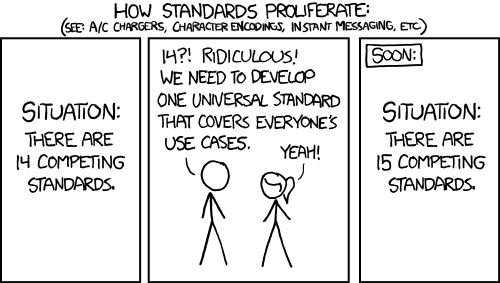
\includegraphics[width=.75\textwidth]{/home/ksipunin/Projects/ling-phd/appl/1-corpora/img/standards.png}
\end{frame}

\subsection{Форматы морфосинтаксической разметки}

\frame{\tableofcontents[currentsection, currentsubsection]}

\begin{frame}[fragile]
    \frametitle{Universal Dependencies}
    \framesubtitle{\autocite{universal_dependencies}}

    \begin{itemize}
        \item >\,200 трибанков на >\,100 языках
        \item Используются для множества NLP-задач, ср.\ библиотеку Stanza
        \item Вместо XML используется CoNLL-U
    \end{itemize}

    \vfill

    \begin{Verbatim}[fontsize=\scriptsize, gobble=8]
        # source = Codex Marianus, Matthew 5
        # text = око за око и зѫбъ за зѫбъ
        # sent_id = 50674
        ID FORM LEMMA UPOS XPOS FEATS HEAD DEPREL DEPS MISC
        1 око око NOUN Nb Case=Acc|Gender=Neut|Number=Sing 0 root 0:root ref=MATT_5.38
        1.1 око око NOUN Nb Case=Acc|Gender=Neut|Number=Sing _ _ 1:conj ref=MATT_5.38
        2 за за ADP R- _ 3 case 3:case ref=MATT_5.38
        3 око око NOUN Nb Case=Acc|Gender=Neut|Number=Sing 1 obl 1:obl:за ref=MATT_5.38
        4 и и CCONJ C- _ 1 cc 1:cc ref=MATT_5.38
        5 зѫбъ зѫбъ NOUN Nb Case=Acc|Gender=Masc|Number=Sing 1 conj 1.1:dep ref=MATT_5.38
        6 за за ADP R- _ 7 case 7:case ref=MATT_5.38
        7 зѫбъ зѫбъ NOUN Nb Case=Acc|Gender=Masc|Number=Sing 5 orphan 1.1:obl:за ref=MATT_5.38
    \end{Verbatim}
\end{frame}

\begin{frame}
    \frametitle{MULTEXT-East}
    \framesubtitle{\autocite{multext_east}}

    \begin{itemize}
        \item Спецификация для 20~языков (используется в TreeTagger)
        \item Лексиконы
        \item Параллельный корпус романа <<1984>> на 12~языках
    \end{itemize}

    \vfill

    \begin{block}{Пример тегсета}
        \textit{он} \linebreak \texttt{P-3msn} \linebreak мест., тип не задан, 3~л., м.~р., ед.~ч., им.~п.
    \end{block}
\end{frame}

\begin{frame}[fragile]
    \frametitle{Syntacticus}
    \framesubtitle{\href{http://dev.syntacticus.org/}{\texttt{dev.syntacticus.org}}}

    \begin{itemize}
        \item Трибанки PROIEL, TOROT и ISWOC на древних языках
        \item Датасеты конвертированы в CoNLL-U
        \item Не поддерживается

    \begin{block}{Пример токена}
        \begin{Verbatim}[fontsize=\scriptsize, gobble=8]
        <token id="674995"
               form="warþ"
               citation-part="MATT 9.25"
               lemma="wairþan"
               part-of-speech="V-"
               morphology="3suia----i"
               head-id="674993"
               relation="pred"
               presentation-after=" "
               foreign-ids="segment_id=143,token_id=2434,witness=CA"
        />
        \end{Verbatim}
    \end{block}
    \end{itemize}
\end{frame}

\subsection{Инструменты}

\frame{\tableofcontents[currentsection, currentsubsection]}

\begin{frame}
    \frametitle{TXM}
    \framesubtitle{\autocite{heiden:2010}, \href{https://txm.gitpages.huma-num.fr/textometrie/en/index.html}{\texttt{txm.gitpages.huma-num.fr}}}

    \begin{itemize}
        \item Корпус-менеджер с текстометрической спецификой
        \item От корпусов речей президентов Франции до древнерусских текстов
        \item Дружит со множеством форматов
    \end{itemize}
\end{frame}

\begin{frame}
    \frametitle{corpus-tools.org}
    \framesubtitle{\autocite{corpus_tools}}

    \begin{itemize}
        \item ANNIS~"--- поиск и визуализация уровней разметки
        \item (Hex)Atomic~"--- многоуровневая разметка
        \item Pepper~"--- конвертация между форматами
        \item Salt~"--- модель данных
    \end{itemize}
\end{frame}

\begin{frame}
    \frametitle{Интерлингва для форматов}
    \centering
    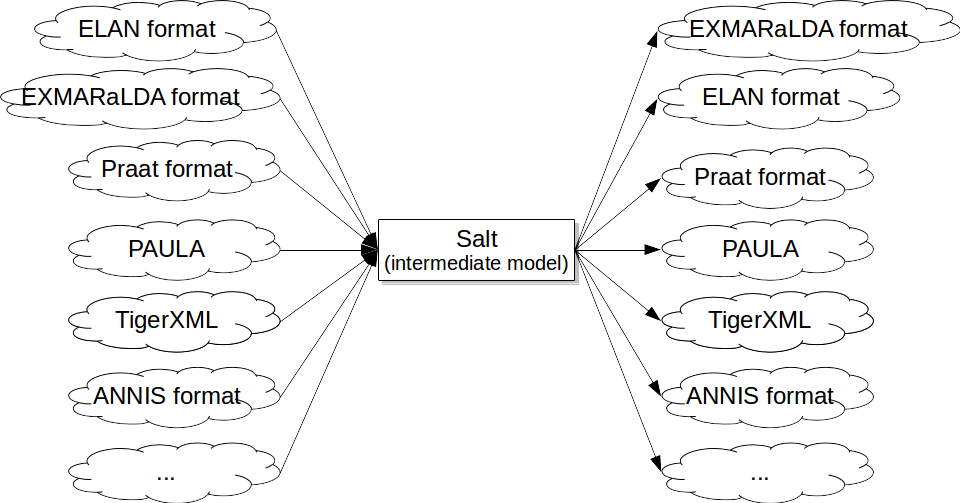
\includegraphics[width=.75\textwidth]{/home/ksipunin/Projects/ling-phd/appl/1-corpora/img/pepper_formats_salt.png}
\end{frame}

\section{Литература}

\frame{\tableofcontents[currentsection]}

\begin{frame}[allowframebreaks]
    \frametitle{Литература}
    \nocite{*}
    \printbibliography
\end{frame}

\begin{frame}{}
    \centering

    \vfill
    Q\&A
    \vfill
\end{frame}

\section{Литература}

\frame{\tableofcontents[currentsection]}

\begin{frame}
    \frametitle{Литература}
    \nocite{*}
    \printbibliography
\end{frame}

\end{document}

